\documentclass[
    a4paper,
    pagesize,
	pdftex,
    12pt,
]{scrartcl}
\usepackage{graphicx} % Required for inserting images
\usepackage[T1]{fontenc}
\usepackage[ngerman]{babel}

\usepackage[unicode=true]{hyperref}
\usepackage[draft=false,babel,tracking=true,kerning=true,spacing=true]{microtype}
\usepackage{enumerate}
\usepackage{fancyhdr}

\graphicspath{{./images/}}

\pagestyle{fancy}
\lhead{Alice, Bob, Charlie} % Bitte auch hier ihre Namen in Form "J. Schroeder"
\rhead{
\includegraphics[height=10mm]{S04_HTW_Berlin_Logo_pos_FARBIG_RGB.jpg}}
\cfoot{\thepage}
\renewcommand{\headrulewidth}{0.6pt}
\renewcommand{\footrulewidth}{0.6pt}

\begin{document}

\begin{titlepage}
    \begin{center}
        
\includegraphics[height=25mm]{S04_HTW_Berlin_Logo_pos_FARBIG_RGB.jpg} \\
        \vspace{1.0cm}

        Ein aussagekräftiger Titel
    
        \vspace{1.5cm}   

        \textbf{Belegarbeit im Modul Informationssicherheit}

        \vspace{1.5cm}

        vorgelegt von \\
        \textbf{Vorname Name Matrikelnr.}%Vor-, Nachname, Matrikelnummer

        \vspace{1.5cm}    
        Berlin, \today\\
    \end{center}
\end{titlepage}

\pagenumbering{gobble}

\thispagestyle{empty}
\tableofcontents
\newpage

\pagenumbering{arabic}

% Nutzen Sie bei jedem neuen Kapitel eine neue Seite \newpage
\section{Einführung}
The software for the ARPA Network exists partly in the IMPs and
partly in the respective HOSTs.  BB\&N has specified the software of
the IMPs and it is the responsibility of the HOST groups to agree on
HOST software. \\ \\
During the summer of 1968, representatives from the initial four
sites met several times to discuss the HOST software and initial
experiments on the network. There emerged from these meetings a
working group of three, Steve Carr from Utah, Jeff Rulifson from SRI,
and Steve Crocker of UCLA, who met during the fall and winter. The
most recent meeting was in the last week of March in Utah. Also
present was Bill Duvall of SRI who has recently started working with
Jeff Rulifson. \\ \\
Somewhat independently, Gerard DeLoche of UCLA has been working on
the HOST-IMP interface. \\ \\
I present here some of the tentative agreements reached and some of
the open questions encountered.  Very little of what is here is firm
and reactions are expected.

\newpage
\section{Bilder, Tabellen, Referenzen}

So werden Bilder eingefügt:

\begin{figure}[!ht]
  \centering
  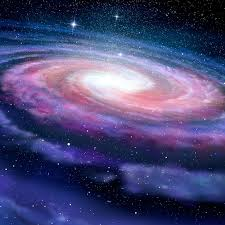
\includegraphics[width=5cm]{milkyway.jpg}
  \caption{Das ist die Milchstraße}
  \label{fig:boat1}
\end{figure}

Eine Referenz auf das Bild folgt über das Label \ref{fig:boat1} oder auf die Tabelle \ref{tab:table1}.

\begin{table}[h!]
  \begin{center}
    \label{tab:table1}
    \begin{tabular}{l|c|r} % <-- Changed to S here.
      \textbf{Value 1} & \textbf{Value 2} & \textbf{Value 3}\\
      $\alpha$ & $\beta$ & $\gamma$ \\
      \hline
      1 & 1110.1 & a\\
      2 & 10.1 & b\\
      3 & 23.113231 & c\\
    \end{tabular}
    \caption{Table with aligned units.}
  \end{center}
\end{table}

Passende Referenzen finden Sie z.B. unter \href{https://dblp.org/}{dblp}. Dort können Sie nach dem Titel des Papers suchen und sich die Bibtex citation rauskopieren. Ein Beispiel finden Sie in der "references.bib"  Datei. Um darauf zuzugreifen, nutzen Sie den folgenden Befehl \cite{scikit-learn}. Wenn es möglich ist, geben Sie noch den Link mit an, wo die Referenz zu finden ist.

% Referenzen bitte in references.bib einfügen
\newpage

\bibliographystyle{ieeetr}
\bibliography{references}

\end{document}
